\documentclass{beamer}

\usepackage{fontspec,xunicode,xltxtra}

\usepackage{tikz}

\XeTeXlinebreaklocale "zh"
\XeTeXlinebreakskip = 0pt plus 1pt minus 0.1pt

%\setmainfont[Mapping=tex-text]{AR PL UMing CN:style=Light}
%\setmainfont[Mapping=tex-text]{AR PL UKai CN:style=Book}
%\setmainfont[Mapping=tex-text]{WenQuanYi Zen Hei:style=Regular}
%\setmainfont[Mapping=tex-text]{WenQuanYi Zen Hei Sharp:style=Regular}
%\setmainfont[Mapping=tex-text]{AR PL KaitiM GB:style=Regular} 
%\setmainfont[Mapping=tex-text]{AR PL SungtiL GB:style=Regular} 
%\setmainfont[Mapping=tex-text]{WenQuanYi Zen Hei Mono:style=Regular} 


\newfontfamily\hei{WenQuanYi Micro Hei}
\newfontfamily\whei{WenQuanYi Zen Hei}
\newfontfamily\kai{AR PL UKai CN}
\newfontfamily\song{AR PL UMing CN}
\newfontfamily\bhei{cwTeXHeiBold}
%\newfontfamily\lishu{SIMLI}
\setmainfont[Mapping=tex-text]{WenQuanYi Micro Hei}
\setsansfont[Mapping=tex-text]{AR PL UKai CN}
\setmonofont[Mapping=tex-text]{WenQuanYi Zen Hei Mono}

\renewcommand{\baselinestretch}{1.25}


\mode<presentation>
{
  \usetheme{Darmstadt}

 % \usetheme{Warsaw}
  % or ...
%  \usetheme{default}

  \setbeamercovered{transparent}
  % or whatever (possibly just delete it)
}


\usepackage[english]{babel}
% or whatever

%\usepackage[latin1]{inputenc}
% or whatever

\title[Beamer + xelatex] % (optional, use only with long paper titles)
{\Huge 数学软件课程总结}

% \subtitle
% {专题一：环境和习惯} % (optional)

\author[Wang HY] % (optional, use only with lots of authors)
{王何宇}
% - Use the \inst{?} command only if the authors have different
%   affiliation.

\institute[ZJU] % (optional, but mostly needed)
{
  浙江大学数学科学学院\\
  信息与计算科学系
}
% - Use the \inst command only if there are several affiliations.
% - Keep it simple, no one is interested in your street address.

\date[] % (optional)
{}


% If you have a file called "university-logo-filename.xxx", where xxx
% is a graphic format that can be processed by latex or pdflatex,
% resp., then you can add a logo as follows:

\pgfdeclareimage[height=1cm]{university-logo}{../images/zju.jpg}
\logo{\pgfuseimage{university-logo}}

% Delete this, if you do not want the table of contents to pop up at
% the beginning of each subsection:
%\AtBeginSubsection[]
%{
%  \begin{frame}<beamer>{Outline}
%    \tableofcontents[currentsection,currentsubsection]
%  \end{frame}
%}


% If you wish to uncover everything in a step-wise fashion, uncomment
% the following command: 

%\beamerdefaultoverlayspecification{<+->}


\begin{document}

\begin{frame}
 \titlepage
\end{frame}

\begin{frame}{提纲}
  \tableofcontents
  % You might wish to add the option [pausesections]
\end{frame}


\section{课程内容回顾}

\begin{frame}{本课主要内容}
  \begin{itemize}
  \item<1-> 课程的主要内容是：
    \begin{itemize}
    \item<1-> 基础的计算机技术，包括一些基本的编程技能。
    \item<1-> 现代数学学习和科研的工作环境的搭建。
    \item<1-> AI 工具的原理和使用。
    \end{itemize}
  \item<2-> 主要目标：高效率地进行数学专业学习和科研。\cite{robbins1951stochastic}
  \end{itemize}
\end{frame}

\begin{frame}{掌握计算机操作技术的必要性}
  \begin{itemize}
  \item<1-> 融入数学科研社区，需要掌握社区普遍接受的科研工具，比如数学排版工具：\LaTeX;
  \item<2-> 学术科研社区在 Linux 环境拥有丰富的开源软件和资源；
  \item<3-> 计算机操作技能也是使用 AI 工具的基础；
  \item<4-> 应用方向的同学需要掌握更多的编程技能，比如 Python, C++, R 等。
  \item<5-> {\color{red} 学习路线的改变：从以文档为中心的学习和练习，到以在 AI 工具的帮助下直接面对任务。}
  \end{itemize}
\end{frame}

\begin{frame}{学习编程的必要性}
  \begin{itemize}
  \item<1-> 我们是否还有必要学习编程？未来是否还有程序员这个工作？
  \item<2-> 对应用数学科研人员来说，编程技能是必不可少的。它是数学模型的实现和验证的基础。
  \begin{itemize}
    \item 高效准确地表达算法;
    \item 编程能优化和检验人类的思考逻辑；
    \item 不必在编程技术的精雕细琢本身上花费过多的精力，脱离具体编程语言的算法和数据结构的学习是更重要的。
  \end{itemize}
  \item<3-> 工业编程呢？码农会消失，但程序设计师不会。
  \item<4-> {\color{red}忠告：不要痴迷于刷 LeetCode。有时间在能学数学的年纪，多学点硬核的数学。}
  \end{itemize}
\end{frame}

\section{使用 AI 工具学习非专业数学}

\begin{frame}{一道例题}
  \begin{itemize}
  \item<1-> 问题描述：求不定积分：
  $$
    \int \frac{1}{x} \sqrt{\frac{x + 1}{x}} \, dx
  $$
  \item<2-> AI 环境：deppseek V3 （不打开深度思考，不联网），官网网页版。
  \item<3-> 以下结果完全由 AI 生成，
  除排版整理外未作任何实质性修改。 
  \end{itemize}
\end{frame}

\begin{frame}{第一步：简化被积函数}
首先，观察被积函数：

$$
\frac{1}{x} \sqrt{\frac{x + 1}{x}}
$$

可以将其简化为：

$$
\frac{1}{x} \sqrt{1 + \frac{1}{x}} = \frac{1}{x} \left(1 + \frac{1}{x}\right)^{1/2}
$$
\end{frame}

\begin{frame}{第二步：变量替换}

为了简化积分，设：
$$
t = 1 + \frac{1}{x}, \quad \text{则} \quad \frac{1}{x} = t - 1
$$
计算微分 ( dt ):
$$
dt = d\left(1 + \frac{1}{x}\right) = -\frac{1}{x^2} dx \quad \Rightarrow \quad dx = -x^2 dt
$$
由于 $\frac{1}{x} = t - 1$，所以 $x = \frac{1}{t - 1}$，因此：
$$
dx = -\frac{1}{(t - 1)^2} dt.
$$
\end{frame}

\begin{frame}{第三步：用新变量表示积分}
将 $\frac{1}{x}$ 和 $dx$ 用 $t$ 表示：
$$
\frac{1}{x} = t - 1, \quad dx = -\frac{1}{(t - 1)^2} dt
$$
因此，积分变为：
$$
\int \frac{1}{x} \sqrt{t} \, dx = \int (t - 1) \sqrt{t} \left(-\frac{1}{(t - 1)^2}\right) dt = -\int \frac{\sqrt{t}}{t - 1} dt
$$
\end{frame}

\begin{frame}{第四步：进一步简化积分}
将 $\sqrt{t}$ 表示为 $t^{1/2}$:
$$
-\int \frac{t^{1/2}}{t - 1} dt
$$
为了消除根号，设：
$$
u = \sqrt{t}, \quad t = u^2, \quad dt = 2u \, du
$$
因此，积分变为：
$$
-\int \frac{u}{u^2 - 1} \cdot 2u \, du = -2 \int \frac{u^2}{u^2 - 1} du
$$
\end{frame}

\begin{frame}{第五步：多项式长除法}
对 $\frac{u^2}{u^2 - 1}$ 进行多项式长除法：
$$
\frac{u^2}{u^2 - 1} = 1 + \frac{1}{u^2 - 1}
$$
因此：
\begin{align*}
&-2 \int \left(1 + \frac{1}{u^2 - 1}\right) du \\
&= -2 \left( \int 1 \, du + \int \frac{1}{u^2 - 1} du \right) \\
&= -2u - 2 \int \frac{1}{u^2 - 1} du
\end{align*}
\end{frame}

\begin{frame}{第六步：计算剩余积分}
积分 $\int \frac{1}{u^2 - 1} du$ 可以通过部分分式分解：
$$
\frac{1}{u^2 - 1} 
= \frac{1}{(u - 1)(u + 1)} 
= \frac{1}{2} \left( \frac{1}{u - 1} - \frac{1}{u + 1} \right)
$$
因此：
$$
\int \frac{1}{u^2 - 1} du = \frac{1}{2} \ln \left| \frac{u - 1}{u + 1} \right| + C
$$
\end{frame}

\begin{frame}{第七步：合并结果}
将所有部分合并：
$$
-2u - 2 \cdot \frac{1}{2} \ln \left| \frac{u - 1}{u + 1} \right| + C 
= -2u - \ln \left| \frac{u - 1}{u + 1} \right| + C
$$
\end{frame}

% \begin{frame}{第八步：回代变量}
% 首先回代 $u = \sqrt{t}$:
% $$
% -2\sqrt{t} - \ln \left| \frac{\sqrt{t} - 1}{\sqrt{t} + 1} \right| + C
% $$
% 然后回代 $t = 1 + \frac{1}{x}$:
% $$
% -2\sqrt{1 + \frac{1}{x}} 
% - \ln \left| \frac{\sqrt{1 + \frac{1}{x}} - 1}{\sqrt{1 + \frac{1}{x}} + 1} \right| + C
% $$
% \end{farme}

\begin{frame}{第八步：回代变量}
首先回代 $u = \sqrt{t}$:
$$
-2\sqrt{t} - \ln \left| \frac{\sqrt{t} - 1}{\sqrt{t} + 1} \right| + C
$$
然后回代 $t = 1 + \frac{1}{x}$:
$$
-2\sqrt{1 + \frac{1}{x}} 
- \ln \left| \frac{\sqrt{1 + \frac{1}{x}} - 1}{\sqrt{1 + \frac{1}{x}} + 1} \right| + C
$$
\end{frame}

\begin{frame}{第九步：简化表达式}
可以进一步简化：
$$
\sqrt{1 + \frac{1}{x}} = \sqrt{\frac{x + 1}{x}} = \frac{\sqrt{x + 1}}{\sqrt{x}}
$$
因此，最终结果为：
$$
-2 \cdot \frac{\sqrt{x + 1}}{\sqrt{x}} 
- \ln \left| \frac{\frac{\sqrt{x + 1}}{\sqrt{x}} - 1}{\frac{\sqrt{x + 1}}{\sqrt{x}} + 1} \right| + C
$$
或者保留原始形式：
$$
-2 \sqrt{\frac{x + 1}{x}} 
- \ln \left| \frac{\sqrt{\frac{x + 1}{x}} - 1}{\sqrt{\frac{x + 1}{x}} + 1} \right| + C
$$
\end{frame}

\begin{frame}{最终答案}
$$
\int \frac{1}{x} \sqrt{\frac{x + 1}{x}} \, dx 
= \boxed{ -2 \sqrt{\frac{x + 1}{x}} 
- \ln \left| \frac{\sqrt{\frac{x + 1}{x}} - 1}{\sqrt{\frac{x + 1}{x}} + 1} \right| + C }
$$
稍微检查一下，就会发现这个不是很简单的积分，deepseek 做的完全正确，而且步骤详细。
除了积分换元稍微有点繁琐，以及最后化简没有特别到位以外，都对。
\end{frame}

\begin{frame}{激活深度思考后的解答}
\begin{itemize}
  \item<1-> 如果打开了深度搜索（千万不要打开联网），那么第一步换元会变成：
令 $u = 1 + \frac{1}{x}$，然后紧接着会有一步换元：
令 $t = \sqrt{u}$.
  \item<2-> 这个很接近人类计算了，熟练的大学生，第一步换元一般是：
令 $t = \sqrt{1 + \frac{1}{x}}$.
  \item<3-> 而最后一步答案，会进一步使用有理化分母，约简为：
$$
\boxed{-2\,\sqrt{\dfrac{x+1}{x}} + 2\,\ln \left(\sqrt{x+1} + \sqrt{x}\right) + C}
$$
\end{itemize}
\end{frame}

\begin{frame}{阶段性总结}
\begin{itemize}
  \item<1-> 深度思考后的答案甚至超过了标准答案！
  该题来自上海交通大学数学系微积分课题组编撰的《微积分》上册，高等教育出版社，
  2008，p. 244, 例 5.50.
  \item<2-> 原题答案是
$$
\boxed{-2\sqrt{\dfrac{x+1}{x}} 
- \ln \left|x\left(\frac{\sqrt{x+1}}{x} - 1\right)^2\right| + C}
$$
  \item<3-> 实际上，我用类似难度的题目反复实验了多次，deepseek 的正确率接近 100\%，
  也就是说，比优秀的人类大学生强。

\end{itemize}
\end{frame}

\begin{frame}{阶段性总结}
\begin{itemize}
  \item<1-> 不止 deepseek，各大 AI 工具在这个级别数学问题上的表现都很好。
  测试了：Kimi, qianwen, gpt-4o 和 gpt o3.
  \item<2-> 第三方平台，如 poe 和 askmanyai 上，表现远不如官网。
  \item<3-> {\color{red}所以我们至少在使用国内 AI 的时候，尽量使用官网。}
\end{itemize}
\end{frame}

\begin{frame}{阶段性总结}
  \begin{itemize}
    \item<1-> 我们还需要训练微积分计算么？
    \item<2-> 需要！因为计算技巧本身可以提高我们对微积分的理解。
    同时，计算在直观建立过程中起着重要的矫正作用，甚至计算本身也是一种直观。
    \item<3-> 但注意在微积分练习时，充分利用 AI 掌握微积分的计算技巧。
    \item<4-> 不必继续追求单纯的微积分技巧。比如所谓的微积分竞赛，
    甚至过于追求技巧的大学生数学竞赛。对人类而言，掌握微积分原理，
    而不是花时间去处理繁琐复杂的积分计算。
  \end{itemize}
\end{frame}

\section{使用 AI 工具学习专业数学：基础问题}

\begin{frame}{数学分析的基础问题}
  \begin{itemize}
    \item<1-> 我们直接参考 cc98 上数学之韵的回忆卷：2023-2024 数学分析 II 期末：
    \item<2-> 问题：求证函数序列 $f_n(x) = \frac{x^2}{x^2 + (1 - n^2x^2)}$ 在区间 $[0,1]$ 上点态收敛但不一致收敛。
    \item<3-> deepseek 出现服务器繁忙，下面的解答来自 qianwen 3，开启深度思考，自动联网。
    \item<4-> 其他 AI 表现：kimi 长思考，gpt-o3 也都能给出正确答案，但 gpt 4o 给出的是错误证明。
    \item<5-> 综合表现确实 Qwen 3 最好，因为它更新最晚。由此可见 AI 的进步是非常快的。
  \end{itemize}
\end{frame}

\begin{frame}{1. 点态收敛性分析}
对任意固定的 $x \in [0,1]$，当 $n \to \infty$ 时，分母为：
$$
x^2 + (1 - n^2x^2) = 1 + x^2 - n^2x^2.
$$

当 $x = 0$: $f_n(0) = \frac{0}{0 + 1} = 0$，显然收敛到 $0$.

当 $x \in (0,1]$: 随着 $n \to \infty$, $n^2x^2$ 主导分母，分母趋向于 $-\infty$，因此：
  $$
  f_n(x) = \frac{x^2}{1 + x^2 - n^2x^2} \to 0.
  $$
综上，极限函数为 $f(x) = 0$，且在 $[0,1]$ 上逐点收敛。
\end{frame}

\begin{frame}{2. 不一致收敛性分析}
\begin{itemize}
  \item<1-> 反例构造法： 取 $x_n = \frac{1}{n} \in [0,1]$，计算 $f_n(x_n)$：
$$
f_n\left(\frac{1}{n}\right) 
= \frac{\left(\frac{1}{n^2}\right)}{\left(\frac{1}{n^2}\right) + \left(1 - n^2 \cdot \frac{1}{n^2}\right)} = \frac{\frac{1}{n^2}}{\frac{1}{n^2} + (1 - 1)} 
= \frac{\frac{1}{n^2}}{\frac{1}{n^2}} 
= 1.
$$
因此，对任意 $n$，存在 $x_n = \frac{1}{n}$ 使得 $|f_n(x_n) - 0| = 1$. 
取 $\varepsilon = \frac{1}{2}$，显然对任意 $N$，当 $n > N$ 时，
存在 $x_n \in [0,1]$ 使得 $|f_n(x_n)| \geq \varepsilon$，故不满足一致收敛的定义。
\item<2-> 余项准则验证： 若 $\lim_{n \to \infty} \sup_{x \in [0,1]} |f_n(x) - 0| \neq 0$，
则不一致收敛。 由于 $\sup_{x \in [0,1]} |f_n(x)| \geq |f_n(1/n)| = 1$，
故极限为 $1 \neq 0$，进一步证明不一致收敛。
\end{itemize}
\end{frame}

\begin{frame}{结论}
\begin{itemize}
  \item<1-> 点态收敛：对任意 $x \in [0,1]$，$f_n(x) \to 0$。
  \item<2-> 不一致收敛：存在反例序列 $x_n = \frac{1}{n}$ 使得 $|f_n(x_n)| = 1$，
  不满足一致收敛条件。
  \item<3-> 因此，函数序列 $f_n(x)$ 在 $[0,1]$ 上点态收敛但不一致收敛。
\end{itemize}
\end{frame}

\begin{frame}{阶段性总结}
  \begin{itemize}
    \item<1-> 对于专业数学的数学分析，主要的 AI 工具在开启了长思考模式后，都能接近完美回答。
    \item<2-> AI 不会一味地迁就你，而是确保有一致的逻辑性。 
    \item<3-> 数学学习的关键在于讨论。那么现在除了教师、助教和同学，AI 提供了一个非常高质量的专业讨论对象。
  \end{itemize}
\end{frame}

\section{使用 AI 工具学习专业数学：进阶问题}

\begin{frame}{实变函数问题}
\begin{itemize}
  \item<1-> cc98 上的回忆卷，2024 春夏的期末卷；
  \item<2-> 设 $E \subset \mathbb{R}$，
  \begin{itemize}
    \item<2-> (1) 叙述可测集的定义；
    \item<2-> (2) 证明外测度为 $0$ 的集必为可测集；
    \item<2-> (3) 证明零测度集若为开集，则必为空集。
  \end{itemize} 
  \item<3-> 显然这是一道考察可测基本定义的基础题。仍然采用Qwen3 深度思考 + 联网。
\end{itemize}
\end{frame}

\begin{frame}{(1) 可测集的定义}

定义：在实数集 $\mathbb{R}$ 中，一个集合 $E$ 被称为勒贝格可测集（简称可测集），
如果对于任意的 $A \subset \mathbb{R}$，满足卡罗特条件：
$$
m^*(A) = m^*(A \cap E) + m^*(A \cap E^c),
$$
其中 $m^*$ 为外测度，$E^c$ 为 $E$ 的补集。
\begin{itemize}
  \item<2-> 复习这种课程，不能只追求答案了，而是要扫清一切概念上的模糊点。比如这里什么是“外测度”？
  \item<3-> 追问：请给出外测度的严格定义。 
\end{itemize}
\end{frame}

\begin{frame}{外测度的严格定义(AI 回复)}
\small
在测度论中，外测度（Outer Measure）是定义在集合上的非负广义实值函数，
用于从外部逼近集合的“大小”（如长度、面积、体积等）。以下是其严格定义：

定义 1（实数轴上的外测度）设 $E \subseteq \mathbb{R}$ 是任意一个实数子集。
定义 $E$ 的勒贝格外测度 $m^*(E)$ 为：
$$
m^*(E) = \inf \left\{ \sum_{i=1}^\infty |I_i| 
\mid E \subseteq \bigcup_{i=1}^\infty I_i \right\},
$$
其中：
\begin{itemize}
  \item $\{I_i\}_{i=1}^\infty$ 是覆盖 $E$ 的可数个开区间；
  \item $|I_i|$ 表示开区间 $I_i$ 的长度（即 $|(a, b)| = b - a$）；
  \item 下确界（infimum）取遍所有可能的覆盖方式。
\end{itemize}  
\end{frame}

\begin{frame}{提问和追问}
  \begin{itemize}
    \item<1-> 检查自己对一个定义是否完善掌握，要善于提问。比如：闭区间 $[a, b]$ 
    如何用一个开区间从外部覆盖逼近，而且长度还恰好是 $b - a$ 呢？
    \item<2-> 这是一个适合在同学之间讨论的问题，但现在也可以和 AI 讨论。
    \item<3-> 追问：$[a, b]$ 的外测度是多少？  
  \end{itemize}
\end{frame}

\begin{frame}{闭区间 $[a, b]$ 的外测度，AI 回复，有节选}
\begin{itemize}
  \item 构造覆盖： 闭区间 $[a, b]$ 可以被一个开区间 $(a - \varepsilon, b + \varepsilon)$ 
  覆盖，其中 $\varepsilon > 0$ 是任意小的正数。该开区间的长度为：
  $$
  (b + \varepsilon) - (a - \varepsilon) = b - a + 2\varepsilon.
  $$
  随着 $\varepsilon \to 0$，覆盖的开区间长度趋近于 $b - a$。
  \item 下确界： 由于闭区间 $[a, b]$ 的长度为 $b - a$，
  而任何覆盖它的开区间总长度不可能小于 $b - a$（否则无法覆盖整个区间），因此：
  $$
  m^*([a, b]) = \inf \left\{ \sum_{k=1}^\infty \ell(I_k) \right\} = b - a.
  $$
\end{itemize}
\end{frame}

\begin{frame}{充分讨论以严格直观}
  \begin{itemize}
    \item<1-> 上面提出具体例子来建立正面直观，是和 AI 讨论的一个很好的方式。 
    \item<2-> 利用 AI 掌握基本概念的过程，适用于各种专业数学领域的学习。
    AI 会不厌其烦地回答我们各种“初等”甚至是“弱智”的问题，并最终使我们获得正确的直观。 
    \item<3-> 下面再主动追问一个反面例子：举一个不可测集的例子。
  \end{itemize}
\end{frame}

\begin{frame}{维塔利集合的构造 I，AI回复}
  \begin{itemize}
    \item 定义等价关系： 在实数区间 $[0, 1]$ 上定义等价关系：
   $$
   x \sim y \quad \text{当且仅当} \quad x - y \in \mathbb{Q}.
   $$
   即，若两个实数 $x$ 和 $y$ 的差是有理数，则它们属于同一类。
    \item 划分等价类： 根据上述等价关系，区间 $[0, 1]$ 被划分为若干互不相交的等价类。例如：
   等价类 $[q]$ 包含所有形如 $q + r$ 的实数，其中 $r \in \mathbb{Q} \cap [-1, 1]$。
  \end{itemize}
\end{frame}

\begin{frame}{维塔利集合的构造 II，AI回复}
  \begin{itemize}
   \item 使用选择公理选取代表元： 从每个等价类中选取一个代表元（选择公理保证这种选取是可能的），
   将所有这些代表元组成的集合记为 $V$。例如，若某个等价类包含 $0.5$ 
   和 $0.5 + \frac{1}{2} = 0.75$，则从该类中任选一个元素（如 $0.5$）加入 $V$。
    \item 构造平移集： 对每个有理数 $q \in \mathbb{Q} \cap [-1, 1]$，定义平移集：
   $$
   V_q = V + q = \{v + q \mid v \in V\}.
   $$
这些平移集 $V_q$ 是互不相交的（因为 $V$ 中的元素来自不同等价类）。  
  \end{itemize}
\end{frame}

\begin{frame}{证明 V 是不可测集 I, AI 完成}
假设 $V$ 是勒贝格可测集，分析其测度 $m(V)$ 的可能情况：
\begin{itemize}
  \item 若 $m(V) > 0$：由于有理数集 $\mathbb{Q} \cap [-1, 1]$ 是可数无限的，
  平移集 $V_q$ 的并集为：
     $$
     [0, 1] \subseteq \bigcup_{q \in \mathbb{Q} \cap [-1, 1]} V_q \subseteq [-1, 2].
     $$
根据勒贝格测度的可数可加性，测度满足：
     $$
     \sum_{q} m(V_q) = \sum_{q} m(V) = \infty.
     $$
但 $[-1, 2]$ 的测度为 $3$，矛盾。
\end{itemize}
\end{frame}

\begin{frame}{证明 V 是不可测集 II, AI 完成}
假设 $V$ 是勒贝格可测集，分析其测度 $m(V)$ 的可能情况：
\begin{itemize}
\item 若 $m(V) = 0$：同样根据可数可加性，测度满足：
     $$
     m\left(\bigcup_{q} V_q\right) = \sum_{q} m(V) = 0.
     $$
但 $[0, 1] \subseteq \bigcup_{q} V_q$，而 $[0, 1]$ 的测度为 $1$，矛盾。
\item 因此，无论 $m(V)$ 是 $0$ 还是正数，都会导致矛盾。故 $V$ 是不可测集。  
\end{itemize}
\end{frame}

\begin{frame}{证明的分析}
  \begin{itemize}
    \item<1-> 初学者可能对这个证明的主要困惑是：$V$ 的构造？$V_q$ 为何是互不相交的？
    \item<2-> 对于第一个疑问，我们可以将思考中的所有动摇的直观都放进去检验，比如追问：
    \begin{itemize}
      \item<3-> $V$ 是 $[0, 1]$ 的子集么？
      \item<4-> $[0, 1]$ 中的全部有理数属于几个等价类？ 
    \end{itemize}
    \item<5-> 而第二个问题，我们也可以将一般的问题，转为一个具体的例子，来降低思维的强度，比如：
    举例说明一下，$V_0$ 和 $V_0.5$ 不相交。
  \end{itemize}
\end{frame}

\begin{frame}{等价类的唯一性，AI 回复}
\begin{itemize}
  \item 等价类的定义：若 $x \sim y$，则 $x$ 和 $y$ 属于同一等价类。
  每个等价类的形式为 $\{x + q \mid q \in \mathbb{Q}\}$。
  \item 维塔利集的构造：$V$ 中的每个元素都是从不同等价类中选取的唯一代表元。
  因此，若 $v_1, v_2 \in V$ 且 $v_1 \neq v_2$，则 $v_1$ 和 $v_2$ 属于不同的等价类。
\end{itemize}
\end{frame}

\begin{frame}{平移集 $V_0$ 和 $V_{0.5}$ 的定义，AI 回复}
\begin{itemize}
  \item $V_0 = V + 0 = V$：即维塔利集本身。
  \item $V_{0.5} = V + 0.5 = \{v + 0.5 \mid v \in V\}$：将 $V$ 中的每个元素右移 $0.5$。
\end{itemize}
\end{frame}

\begin{frame}{不相交的证明，AI 回复，有节选}
假设存在一个元素 $x$ 同时属于 $V_0$ 和 $V_{0.5}$，即：
$$
x \in V_0 \cap V_{0.5}.
$$
这意味着：
$$
x = v_1 + 0 \quad \text{且} \quad x = v_2 + 0.5, \quad \text{其中 } v_1, v_2 \in V.
$$
由此可得：
$$
v_1 = v_2 + 0.5 \quad \Rightarrow \quad v_1 - v_2 = 0.5.
$$
由于 $0.5 \in \mathbb{Q}$，根据等价关系的定义，$v_1 \sim v_2$，
即 $v_1$ 和 $v_2$ 属于同一等价类。然而，这与维塔利集 $V$ 的构造矛盾  
\end{frame}

\begin{frame}{为什么 $V$ 是不可测的，AI 回复}
  \small
  \begin{itemize}
    \item 不可测性的核心矛盾：若 $V$ 是可测的，则所有平移集 $V_q$ 的测度均为 $m(V)$，
且互不相交。根据可数可加性：
  $$
  m\left(\bigcup_{q \in \mathbb{Q} \cap [-1, 1]} V_q\right) = \sum_{q} m(V).
  $$
  但 $\bigcup V_q$ 覆盖 $[0, 1]$，其测度为 $1$；同时 $\bigcup V_q$ 最多覆盖 $[-1, 2]$，其测度为 3。因此：
  $$
  1 \leq \sum_{q} m(V) \leq 3.
  $$
  若 $m(V) > 0$，则 $\sum m(V) = \infty$，矛盾；若 $m(V) = 0$，则 $\sum m(V) = 0$，矛盾。因此 $V$ 不可测。
  \item 个人分析：$\cup V_q$ 相当于可列个互不相交 $\aleph_1$ 集合的并，因此测度无穷。
  \end{itemize}
\end{frame}

% \begin{frame}{AI 完成一道非专业数学题的例子}
%   \begin{columns}[t]
%   \begin{column}{.5\textwidth}
%   \begin{itemize}
%   \item<1-> 科研和学习的起点是选择文献. 
%   \item<2-> 如何精度一篇论文（\hei{相当个人}）\cite{robbins1951stochastic}。
%   \item<3-> 和大模型进行数学讨论。
%   \item<4-> 模拟和验证论文的结果。
%   \item<5-> 总结和记录讨论的内容。
%   \end{itemize}
% \end{column}
% \begin{column}{.5\textwidth}
%   \begin{figure}
%     \centering
%     \includegraphics<1>[width=0.75\textwidth]{../images/ruby_paper.PNG}
%     \includegraphics<2>[width=0.75\textwidth]{../images/good_paper.PNG}
%     \includegraphics<3>[width=0.75\textwidth]{../images/Aidiot.PNG}
%     \includegraphics<4>[width=0.75\textwidth]{../images/sgd.PNG}
%     \includegraphics<5>[width=0.75\textwidth]{../images/report.PNG}
%   \end{figure}
% \end{column}
% \end{columns}
% \end{frame}

% \begin{frame}{工作环境介绍}
%   \begin{itemize}
%   \item<1-> 大模型的选择：GPT*, Qianwen, Deepseek（有校内版）, kimi, 综合平台, ...
%   \item<2-> 操作系统：Windows 11 + wsl 2, 事实上不重要，需要一个 linux 终端环境.
%   \item<3-> 编辑器：vscode.
%   \item<4-> 项目管理：git. 平台：github, gitee, zjugit, ...
%   \end{itemize}
% \end{frame}


% \begin{frame}{工作环境介绍}
%   \begin{columns}[c]
% % create the column with the first image, that occupies
% % half of the slide
%     \begin{column}{.5\textwidth}
%       \begin{itemize}
%       \item<1-> 繁华下的真像: 二进制流. 
%       \item<2-> 控制计算机, 而不是被控制.
%       \item<3-> core 归计算机, shell 归愚蠢的人类.
%       \item<4-> 掌握了 Terminal/shell, 才能真正掌握计算机(才怪).
%       \end{itemize}
%     \end{column}
% % create the column with the second image, that also
% % occupies half of the slide
%     \begin{column}{.5\textwidth}
%     \begin{figure}
%         \centering
%         \includegraphics<1->[width=0.75\textwidth]{../images/matrix.bmp}
%         \includegraphics<2->[width=0.75\textwidth]{../images/matrixbin.png}
%     \end{figure}
%     \end{column}
% \end{columns}
%   %% \begin{tikzpicture}
%   %%   \node (img1) {\includegraphics[height=3cm]{res/matrix.bmp}};
%   %% \end{tikzpicture}
% \end{frame}

% \begin{frame}{文本编辑器}
%   \begin{itemize}
%   \item<1-> 能基本上完全用键盘控制.
%   \item<2-> 适合终端和 shell 的模式, 不占用太多的软硬件和通讯资源.
%   \item<3-> 能快速高效地发送和接受指令, 完成编码.
%   \item<4-> 推荐: emacs, vim, vscode.
%   \item<5-> 选择一款最适合你自己, 能把你的工作效率提到最高的编辑器.
%   \item<6-> 如果你还是新手, 请盲从大佬.
%   \item<7-> 切记一切以效率为中心, 不要对编辑器提太多不切实际的要求.
%   \item<8-> 如果你不知道怎么配置你的编辑器, 用缺省配置, 或者像同行要一个配置文件. 
%   \end{itemize}
% \end{frame}

% \section{数学写作}
% \begin{frame}{如何产生漂亮的数学文章}
%   \begin{tikzpicture}[remember picture, overlay]
%     \node[left = 2cm, above = -0.1cm] at (current page.east) 
%          {
%            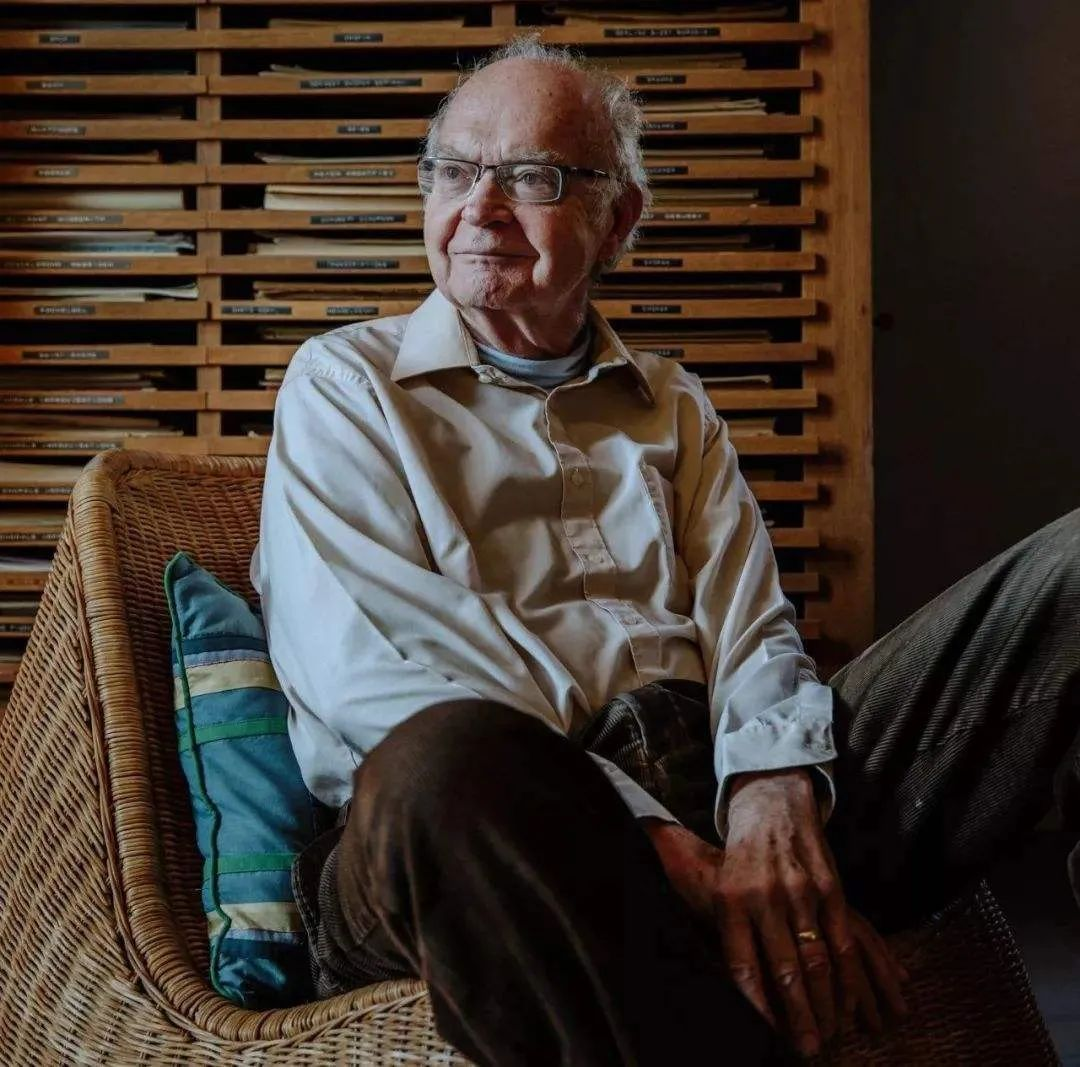
\includegraphics[width=0.25\textwidth]{../images/knuth.png}
%          };
% \end{tikzpicture}  
%   \begin{itemize}
%   \item<1-> 数学家对写作有特殊的要求.
%   \item<2-> 同样必须满足键盘, 终端和高效的原则.
%   \item<3-> 唯一解也是事实上的标准: \LaTeX.
%   \item<4-> 参考资料: lshort, manual, ...
%   \item<5-> 去找一个例子.
%   \item<6-> 必须亲自动手写点什么. 
%   \end{itemize}
% \end{frame}

% \begin{frame}{Latex进阶}
%   \begin{itemize}
%   \item<1-> 交叉引用和计数器.
%   \item<2-> 图, 表和正文混排.
%   \item<3-> 报告的制作.
%   \item<4-> 手工绘图.
%   \end{itemize}
% \end{frame}

% \begin{frame}{作业：设置你的工作环境}
%   \begin{itemize}
%   \item<1-> 选择并熟悉你的大语言模型，可以不止一个。
%   \item<2-> 准备一个 linux 环境，可以是 wsl 2, 也可以是虚拟机.
%   \item<3-> 选择并安装配置一个编辑器，推荐 vscode. 
%   \item<4-> 注册一个作业 git 账号，熟悉 git 的基本操作.
%   \item<5-> 在作业包中两本经典教材中选择一本，根据你的兴趣选择一个主要定理的叙述和证明，加上你自己的理解，写成一份报告.
%   \end{itemize}
% \end{frame}

\bibliography{../mathsoft.bib}
\bibliographystyle{plain}
\end{document}


